\documentclass[12pt]{article}

\usepackage[spanish]{babel}
\usepackage[none]{hyphenat}
\usepackage[left=1.5cm, right=1.5cm, top = 2cm, bottom=2.5cm]{geometry}
\usepackage{parskip}
\usepackage[export]{adjustbox}
\usepackage{enumitem}[shortlabels]
\usepackage{listings} 
\usepackage{color}
\usepackage{fancyhdr}
\usepackage{graphicx}
\usepackage{caption} 
% \usepackage{subcaption}
\usepackage{wrapfig}
% \usepackage{longtable}
% \usepackage{multirow, makecell}
% \usepackage{amsmath} 
\usepackage[hidelinks]{hyperref}
\usepackage{csquotes}

\newcommand{\linejump}{\hfill \break}
\renewcommand{\thefootnote}{\fnsymbol{footnote}}
% \newcommand{\unit}[1]{\ensuremath{\, \mathrm{#1}}}

\definecolor{dkgreen}{rgb}{0,0.6,0}
\definecolor{gray}{rgb}{0.5,0.5,0.5}
\definecolor{mauve}{rgb}{0.58,0,0.82}
\lstset{
  language=Java,
  aboveskip=3mm,
  belowskip=3mm,
  showstringspaces=false,
  columns=flexible,
  basicstyle={\scriptsize\ttfamily},
  numbers=none,
  numberstyle=\tiny\color{gray},
  keywordstyle=\color{blue},
  commentstyle=\color{dkgreen},
  stringstyle=\color{mauve},
  breaklines=true,
  breakatwhitespace=true,
  tabsize=2
}

\sloppy
\setlength{\parindent}{0cm}
\setlength{\columnsep}{0.5cm}
\decimalpoint
\graphicspath{{img/}}

\hypersetup{colorlinks=true, urlcolor=blue, citecolor=blue}
\urlstyle{same}

\pagestyle{fancyplain}
\fancyhf{}
\fancyhead[L]{\scriptsize 
  National Autonomous University of Mexico \\
  Object Oriented Programming \\
  M.C. Leonardo Ledesma Dominguez
}
\fancyhead[R]{\thepage}


\begin{document}
  \begin{center}
    Acosta Porcayo Alan Omar, Gutiérrez Grimaldo Alejandro, Medina Villa Samuel, Valera Jiménez Diego, Zarza Zurita Axel Zahir \\
    \linejump
    \LARGE \textbf{Research project. Conway's Game of Life} \\
  \end{center}

  \section*{Team members}
  Acosta Porcayo Alan Omar 320206102 \\
  Gutiérrez Grimaldo Alejandro 320282098 \\
  Medina Villa Samuel 320249538 \\
  Valera Jiménez Diego 320013447 \\
  Zarza Zurita Axel Zahir 316075842

  \section*{Breef description and historical background}
  Interest in cellular automata in general dates back to the 1940's and 1950's when mathematicians like John von Neumann and Stanislaw Ulam began exploring discrete systems that evolve in discrete steps based on local rules. 
  
  These early works laid the groundwork for the development of Conway's Game of Life, which became one of the most iconic examples of cellular automata. Its creation and popularization are primarily credited to John Conway, who managed to capture the attention of both the mathematical community and the general public due to its simplicity and the complex structures that can emerge from it.
  
  \begin{wrapfigure}{r}{0.4\columnwidth}
    \centering
    
\includegraphics[width=\linewidth, center]{conway.jpg}
  \end{wrapfigure}
  
  Conway's Game of Life is a mathematical simulation game created by British mathematician John Conway in 1970. It is played on a two-dimensional grid of cells, where each cell can be alive or dead. The evolution of the game is based on simple rules that determine the state of each cell based on its neighbors. If a cell has too few or too many live neighbors, it dies; if a dead cell has exactly three live neighbors, a new cell is born in that position. These simple rules give rise to a wide variety of patterns and behaviors, ranging from static structures to oscillators and spaceships.
  

  Despite its simplicity, Conway's Game of Life has been used as a model to explore concepts in computer theory and nonlinear dynamics. It has been found to be equivalent to a universal Turing machine, meaning it can be used to simulate any computational process. Furthermore, the game has inspired research in various disciplines, from biology and physics to mathematics and computer science.

  \section*{OOP Interpretability}
  \subsection*{Class and objects}
  \begin{itemize}
    \item \textbf{GameOfLife class}: This is the main class of the program, which inherits from the \textit{JFrame} class and implements the \textit{ActionListener} interface. The attributes of this class are mostly a combination of other classes, such as the \textit{Dimension} object, \textit{JMenuBar, JMenu, JMenuItem, Thread}, and \textit{GameBoard}, which is a class defined within the \textit{GameOfLife} class itself. The methods of this class are defined to initialize the program by creating the window with menus that allow interaction and detecting user actions.

    \item \textbf{GameBoard class}: This second class, which is also defined within the \textit{GameOfLife} class, inherits from \textit{JPanel} and implements \textit{ComponentListener, MouseListener, MouseMotionListener}, and \textit{Runnable}. This class contains the core logic of the program, utilizing objects such as \textit{Dimension} and the \textit{ArrayList} collection. The methods implemented in this class allow us to add points to the grid, fill the grid randomly, and apply the rules of the Game of Life as previously explained. Additionally, this class utilizes the functionality of Threads and the Try-Catch structure for exception handling.
  \end{itemize}

  \subsection*{Inheritance}
  \begin{itemize}
    \item \textbf{JFrame:} \textit{GameOfLife} class inherits from \textit{JFrame} to create a graphical user interface for the game.
    \item \textbf{JPanel:} The \textit{GameBoard} class inherits from the \textit{JPanel} class to create the game board, where the cells of the Game of Life are displayed.
  \end{itemize}

  \subsection*{Interfaces}
  \begin{itemize}
    \item \textbf{ActionListener:} The \textit{GameOfLife} class implements the ActionListener interface to handle user actions like button clicks and menu selections.
    \item \textbf{ComponentListener:} This interface allows the \textit{GameBoard} class to listen for component-related events, such as resizing the window.
    \item \textbf{MouseListener and MouseMotionListener:} These interfaces enable the \textit{GameBoard} class to listen for mouse-related events, including clicks, releases, and drag actions. 
    \item \textbf{Runnable:} By implementing the \textit{Runnable} interface, the \textit{GameBoard} class can be executed as a separate thread, which is responsible for running the Game of Life simulation.
  \end{itemize}

  \subsection*{Polymorphism}
  \begin{itemize}
    \item \textit{paintComponent(Graphics g)} method is overridden to customize how the game board is painted. This method is originally defined in the \textit{JPanel} class.
    \item Methods such as \textit{componentResized(ComponentEvent e)}, \textit{mouseClicked(MouseEvent e)}, \textit{mousePressed(MouseEvent e)}, and others are overridden to provide specific behavior for each event.
    \item The \textit{actionPerformed(ActionEvent ae)} method in the \textit{GameOfLife} class handles different actions triggered by menu items. It uses the \textit{ActionEvent} parameter to determine the source of the action which allows it to perform different actions based on the source.
    \item The interfaces implemented enables the class to provide specific implementations for the methods required by these interfaces. For example, it overrides \textit{run()} as part of the \textit{Runnable} interface to define the simulation logic.
    \item The game thread is created as new \textit{Thread(gb$\_$gameBoard)}. It references the \textit{gb$\_$gameBoard} object, which is an instance of the \textit{GameBoard} class. This demonstrates polymorphism, as the \textit{Thread} class can work with any object that implements the \textit{Runnable} interface.
  \end{itemize}

  \section*{Coding}
  \subsection*{Code}
  \begin{lstlisting}
import java.awt.*;
import java.awt.event.*;
import java.util.ArrayList;
import java.util.ConcurrentModificationException;
import javax.swing.*;
import java.net.URI;

import java.io.File;

import javax.sound.sampled.AudioFileFormat;
import javax.sound.sampled.AudioSystem;
import javax.sound.sampled.Clip;

public class GameOfLife extends JFrame implements ActionListener {
  private static final Dimension DEFAULT_WINDOW_SIZE = new Dimension(800, 600);
  private static final Dimension MINIMUM_WINDOW_SIZE = new Dimension(400, 400);
  private static final int BLOCK_SIZE = 10;

  private final JMenuBar mb_menu;
  private final JMenu m_file;
  private final JMenu m_game;
  private final JMenu m_help;
  private final JMenuItem mi_file_options;
  private final JMenuItem mi_file_exit;
  private final JMenuItem mi_game_play;
  private final JMenuItem mi_game_autofill;
  private final JMenuItem mi_game_stop;
  private final JMenuItem mi_game_reset;
  private final JMenuItem mi_help_about;
  private int i_movesPerSecond = 3;
  private final GameBoard gb_gameBoard;
  private Thread game;

  public static void main(String[] args) {
    JFrame game = new GameOfLife();
    game.setDefaultCloseOperation(JFrame.EXIT_ON_CLOSE);
    game.setTitle("Conway's Game of Life");
    ImageIcon img = new ImageIcon("logo.png");
    game.setIconImage(img.getImage());
    game.setSize(DEFAULT_WINDOW_SIZE);
    game.setMinimumSize(MINIMUM_WINDOW_SIZE);
    game.setLocation((Toolkit.getDefaultToolkit().getScreenSize().width - game.getWidth()) / 2,
        (Toolkit.getDefaultToolkit().getScreenSize().height - game.getHeight()) / 2);
    game.setVisible(true);
  }

  public GameOfLife() {
    mb_menu = new JMenuBar();
    setJMenuBar(mb_menu);
    m_file = new JMenu("File");
    mb_menu.add(m_file);
    m_game = new JMenu("Game");
    mb_menu.add(m_game);
    m_help = new JMenu("Help");
    mb_menu.add(m_help);

    mi_file_options = new JMenuItem("Options");
    mi_file_options.addActionListener(this);
    mi_file_exit = new JMenuItem("Exit");
    mi_file_exit.addActionListener(this);
    m_file.add(mi_file_options);
    m_file.add(new JSeparator());
    m_file.add(mi_file_exit);
    mi_game_autofill = new JMenuItem("Autofill");
    mi_game_autofill.addActionListener(this);
    mi_game_play = new JMenuItem("Play");
    mi_game_play.addActionListener(this);
    mi_game_stop = new JMenuItem("Stop");
    mi_game_stop.setEnabled(false);
    mi_game_stop.addActionListener(this);
    mi_game_reset = new JMenuItem("Reset");
    mi_game_reset.addActionListener(this);
    m_game.add(mi_game_autofill);
    m_game.add(new JSeparator());
    m_game.add(mi_game_play);
    m_game.add(mi_game_stop);
    m_game.add(mi_game_reset);
    mi_help_about = new JMenuItem("About");
    mi_help_about.addActionListener(this);
    m_help.add(mi_help_about);

    gb_gameBoard = new GameBoard();
    add(gb_gameBoard);

    try {
      Clip sonido = AudioSystem.getClip();
      sonido.open(AudioSystem.getAudioInputStream(new File("TheMandalorian.wav")));
      sonido.start();
    } catch (Exception e) {
      System.out.println("" + e);
    }
  }

  public void setGameBeingPlayed(boolean isBeingPlayed) {
    if (isBeingPlayed) {
      mi_game_play.setEnabled(false);
      mi_game_stop.setEnabled(true);
      game = new Thread(gb_gameBoard);
      game.start();
    } else {
      mi_game_play.setEnabled(true);
      mi_game_stop.setEnabled(false);
      game.interrupt();
    }
  }

  @Override
  public void actionPerformed(ActionEvent ae) {
    if (ae.getSource().equals(mi_file_exit)) {
      System.exit(0);
    } else if (ae.getSource().equals(mi_file_options)) {
      final JFrame f_options = new JFrame();
      f_options.setTitle("Options");
      f_options.setSize(300, 100);
      f_options.setLocation((Toolkit.getDefaultToolkit().getScreenSize().width - f_options.getWidth()) / 2,
          (Toolkit.getDefaultToolkit().getScreenSize().height - f_options.getHeight()) / 2);
      f_options.setResizable(false);
    \textit{  JPanel} p_options = new JPanel();
      p_options.setOpaque(false);
      f_options.add(p_options);
      p_options.add(new JLabel("Number of moves per second:"));
      Integer[] secondOptions = { 1, 2, 3, 4, 5, 10, 15, 20 };
      final JComboBox cb_seconds = new JComboBox(secondOptions);
      p_options.add(cb_seconds);
      cb_seconds.setSelectedItem(i_movesPerSecond);
      cb_seconds.addActionListener(new ActionListener() {
        @Override
        public void actionPerformed(ActionEvent ae) {
          i_movesPerSecond = (Integer) cb_seconds.getSelectedItem();
          f_options.dispose();
        }
      });
      f_options.setVisible(true);
    } else if (ae.getSource().equals(mi_game_autofill)) {
      final JFrame f_autoFill = new JFrame();
      f_autoFill.setTitle("Autofill");
      f_autoFill.setSize(360, 60);
      f_autoFill.setLocation((Toolkit.getDefaultToolkit().getScreenSize().width - f_autoFill.getWidth()) / 2,
          (Toolkit.getDefaultToolkit().getScreenSize().height - f_autoFill.getHeight()) / 2);
      f_autoFill.setResizable(false);
      JPanel p_autoFill = new JPanel();
      p_autoFill.setOpaque(false);
      f_autoFill.add(p_autoFill);
      p_autoFill.add(new JLabel("What percentage should be filled? "));
      Object[] percentageOptions = { "Select", 5, 10, 15, 20, 25, 30, 40, 50, 60, 70, 80, 90, 95 };
      final JComboBox cb_percent = new JComboBox(percentageOptions);
      p_autoFill.add(cb_percent);
      cb_percent.addActionListener(new ActionListener() {
        @Override
        public void actionPerformed(ActionEvent e) {
          if (cb_percent.getSelectedIndex() > 0) {
            gb_gameBoard.resetBoard();
            gb_gameBoard.randomlyFillBoard((Integer) cb_percent.getSelectedItem());
            f_autoFill.dispose();
          }
        }
      });
      f_autoFill.setVisible(true);
    } else if (ae.getSource().equals(mi_game_reset)) {
      gb_gameBoard.resetBoard();
      gb_gameBoard.repaint();

    } else if (ae.getSource().equals(mi_game_play)) {
      setGameBeingPlayed(true);
    } else if (ae.getSource().equals(mi_game_stop)) {
      setGameBeingPlayed(false);
    }

    else if (ae.getSource().equals(mi_help_about)) {
      Desktop desktop = Desktop.isDesktopSupported() ? Desktop.getDesktop() : null;
      try {
        desktop.browse(new URI("https://www.youtube.com/watch?v=OWXD_wJxCKQ"));
      } catch (Exception ex) {
        JOptionPane.showMessageDialog(null,
            "Conway's game of life was a cellular animation devised by the mathematician John Conway", "Source",
            JOptionPane.INFORMATION_MESSAGE);
      }
    }
  }

  private class GameBoard extends JPanel implements ComponentListener, MouseListener, MouseMotionListener, Runnable {
    private Dimension d_gameBoardSize = null;
    private final ArrayList<Point> point = new ArrayList<Point>(0);

    public GameBoard() {
      addComponentListener(this);
      addMouseListener(this);
      addMouseMotionListener(this);
    }

    public void resetBoard() {
      point.clear();
    }

    private void updateArraySize() {
      ArrayList<Point> removeList = new ArrayList<Point>(0);
      for (Point current : point) {
        if ((current.x > d_gameBoardSize.width - 1) || (current.y > d_gameBoardSize.height - 1)) {
          removeList.add(current);
        }
      }
      point.removeAll(removeList);
      repaint();
    }

    public void removePoint(int x, int y) {
      point.remove(new Point(x, y));
    }

    public void addPoint(int x, int y) {
      if (!point.contains(new Point(x, y))) {
        point.add(new Point(x, y));
      }
      repaint();
    }

    public void addPoint(MouseEvent me) {
      int x = me.getPoint().x / BLOCK_SIZE - 1;
      int y = me.getPoint().y / BLOCK_SIZE - 1;
      if ((x >= 0) && (x < d_gameBoardSize.width) && (y >= 0) && (y < d_gameBoardSize.height)) {
        addPoint(x, y);
      }
    }

    public void randomlyFillBoard(int percent) {
      for (int i = 0; i < d_gameBoardSize.width; i++) {
        for (int j = 0; j < d_gameBoardSize.height; j++) {
          if (Math.random() * 100 < percent) {
            addPoint(i, j);
          }
        }
      }
    }

    @Override
    public void paintComponent(Graphics g) {
      super.paintComponent(g);
      try {
        for (Point newPoint : point) {
          g.setColor(Color.blue);
          g.fillRect(BLOCK_SIZE + (BLOCK_SIZE * newPoint.x), BLOCK_SIZE + (BLOCK_SIZE * newPoint.y), BLOCK_SIZE,
              BLOCK_SIZE);
        }
      } catch (ConcurrentModificationException cme) {}

      g.setColor(Color.BLACK);
      for (int i = 0; i <= d_gameBoardSize.width; i++) {
        g.drawLine(((i * BLOCK_SIZE) + BLOCK_SIZE), BLOCK_SIZE, (i * BLOCK_SIZE) + BLOCK_SIZE,
            (BLOCK_SIZE * d_gameBoardSize.height));
      }

      for (int i = 0; i <= d_gameBoardSize.height; i++) {
        g.drawLine(BLOCK_SIZE, ((i * BLOCK_SIZE) + BLOCK_SIZE), (BLOCK_SIZE * d_gameBoardSize.width + 1),
            ((i * BLOCK_SIZE) + BLOCK_SIZE));
      }
    }

    @Override
    public void componentResized(ComponentEvent e) {
      d_gameBoardSize = new Dimension(getWidth() / BLOCK_SIZE - 2, getHeight() / BLOCK_SIZE - 2);
      updateArraySize();
    }

    @Override
    public void componentMoved(ComponentEvent e) {}

    @Override
    public void componentShown(ComponentEvent e) {}

    @Override
    public void componentHidden(ComponentEvent e) {}

    @Override
    public void mouseClicked(MouseEvent e) {}

    @Override
    public void mouseReleased(MouseEvent e) {
      addPoint(e);
    }

    @Override
    public void mousePressed(MouseEvent e) {}

    @Override
    public void mouseExited(MouseEvent e) {}

    @Override
    public void mouseEntered(MouseEvent e) {}

    @Override
    public void mouseDragged(MouseEvent e) {
      addPoint(e);
    }

    @Override
    public void mouseMoved(MouseEvent e) {}

    @Override
    public void run() {
      boolean[][] gameBoard = new boolean[d_gameBoardSize.width + 2][d_gameBoardSize.height + 2];
      for (Point current : point) {
        gameBoard[current.x + 1][current.y + 1] = true;
      }

      ArrayList<Point> survivingCells = new ArrayList<Point>(0);

      for (int i = 1; i < gameBoard.length - 1; i++) {
        for (int j = 1; j < gameBoard[0].length - 1; j++) {
          int surrounding = 0;
          if (gameBoard[i - 1][j - 1]) {
            surrounding++;
          }
          if (gameBoard[i - 1][j]) {
            surrounding++;
          }
          if (gameBoard[i - 1][j + 1]) {
            surrounding++;
          }

          if (gameBoard[i][j - 1]) {
            surrounding++;
          }
          if (gameBoard[i][j + 1]) {
            surrounding++;
          }

          if (gameBoard[i + 1][j - 1]) {
            surrounding++;
          }
          if (gameBoard[i + 1][j]) {
            surrounding++;
          }
          if (gameBoard[i + 1][j + 1]) {
            surrounding++;
          }

          if (gameBoard[i][j]) {
            if ((surrounding == 2) || (surrounding == 3)) {
              survivingCells.add(new Point(i - 1, j - 1));
            }
          } else {
            if (surrounding == 3) {
              survivingCells.add(new Point(i - 1, j - 1));
            }
          }

        }
      }

      resetBoard();
      point.addAll(survivingCells);
      repaint();

      try {
        Thread.sleep(1000 / i_movesPerSecond);
        run();
      } catch (InterruptedException e) {}
    }
  }
}
  \end{lstlisting}

  \subsection*{UML Scheme}
  \begin{figure}[ht]
    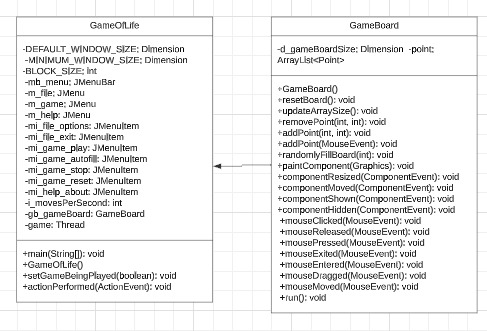
\includegraphics[center]{uml.jpg}
  \end{figure}

  \subsection*{Relevant features}
  \begin{itemize}
    \item \textbf{Start/Play}: Begin the game simulation.
    \item \textbf{Pause/Stop}: Pause or stop the game simulation.
    \item \textbf{Reset}: Reset the game board to its initial state.
    \item \textbf{Add Cells}: Allow users to add or place cells on the game board.
    \item \textbf{Remove Cells}: Allow users to remove cells from the game board.
    \item \textbf{Menus}: Implement menus for game control and options.
    \item \textbf{About}: Provide basic information about the game and its rules.
    \item \textbf{Optimization}: Optimize the game engine for better performance.
  \end{itemize}

  \subsection*{Functionalty core}
  \begin{itemize}
    \item \textbf{Game Board}: Display a grid-based game board where cells can live or die according to the rules of Conway's Game of Life.
    \item \textbf{Cell Interaction}: Allow users to add or remove cells from the grid.
    \item \textbf{Remove Cells}: Enable users to remove cells from the grid.
    \item \textbf{Start/Play}: Initiate the simulation to observe the evolution of cells over time.
    \item \textbf{Pause/Stop}: Pause or stop the simulation to make changes or analyze the current state.
    \item \textbf{Rule Implementation}: Implement the rules of Conway's Game of Life, where cells live, die, or reproduce based on the number of neighboring cells.
    \item \textbf{Simulation Speed}: Allow users to control the speed of the simulation, such as setting the generation update interval.
    \item \textbf{Reset}: Provide an option to reset the game board to its initial state.
    \item \textbf{User Interface}: Simple and intuitive user interface for interacting with the game board.
  \end{itemize}

  \subsection*{Exception classification}
  \begin{itemize}
    \item \textbf{\textit{IOException} (java.io.IOException)}: This exception could be raised when attempting to open and play the audio file "TheMandalorian.wav" using \textit{AudioSystem}. 

    \textbf{Handling:} The code has a try-catch block to catch exceptions when working with the audio file. If an exception occurs, it prints the exception message to the console.
    \item \textbf{\textit{ConcurrentModificationException} (java.util.ConcurrentModificationException)}: This exception can occur when iterating over the point \textit{ArrayList} while simultaneously modifying it. It's a common issue when using a non-thread-safe collection in a multi-threaded environment.
    
    \textbf{Handling:} The code has a try-catch block around the iteration over the point \textit{ArrayList} in the paintComponent method. If this exception occurs, it is caught and ignored.
    \item \textbf{NullPointerException (java.lang.NullPointerException)}: There could be a potential \textit{NullPointerException} when using the Desktop object in the actionPerformed method. If the Desktop object is not supported on the platform or the URI is invalid, a \textit{NullPointerException} may be thrown.
    
    \textbf{Handling:} The code checks if Desktop is supported before using it. If it's not supported, it displays an \textit{JOptionPane} message with information about Conway's Game of Life.
    \item \textbf{InterruptedException (java.lang.InterruptedException)}: The run method in the \textit{GameBoard} class explicitly throws an \textit{InterruptedException} without handling it.
    
    \textbf{Handling:} To properly handle the \textit{InterruptedException}, you should surround the run method's contents with a try-catch block to catch and handle this exception.
  \end{itemize}

  \section*{Possible improvements / Adding ideas}
  \begin{itemize}
    \item \textbf{Adding more dimensions:} The Game of Life is currently played on a two-dimensional grid. Adding an additional dimension could lead to even more complex patterns and shapes. For example, a three-dimensional grid could allow for the creation of floating or moving structures.
    \item \textbf{Adding objectives:} Objectives could be added to the Game of Life, such as reaching a certain number of live cells or creating a specific pattern. This could make the game more challenging and strategic.
  \end{itemize}

  \section*{References}
  Derivando. (n.d.). \textit{¿Conoces el juego de la vida de Conway?} [Video]. YouTube. \url{https://www.youtube.com/watch?v=OWXD_wJxCKQ&ab_channel=Derivando} \\

  \textit{Juego de la vida}. (n.d.). \url{https://complejidad.iiec.unam.mx/cursotaller2020/mba/juegoVida.php} \\

  Mike, M. (n.d.). \textit{EL JUEGO DE LA VIDA DE CONWAY} [Video]. YouTube. \url{https://www.youtube.com/watch?v=2ssnMkJFqbA&ab_channel=MatesMike} \\

  Morgan. (2022). Conway. El Juego de la Vida. \textit{ADNTRO}. \url{https://adntro.com/es/blog/noticias-corporativas/conway/} \\

  Numberphile. (n.d.). \textit{Inventing Game of Life (John Conway) - Numberphile} [Video]. YouTube. \url{https://www.youtube.com/watch?v=R9Plq-D1gEk&ab_channel=Numberphile}
\end{document}